\chapter{Hyperledger Fabric}
\label{ch:Fabric}
Hyperledger Fabric \cite{androulaki2018hyperledger} is a framework to create permissioned distributed ledger networks, open source and hosted under the Linux Foundation, with major contributions from IBM, Digital Asset and Secure key, among others. It is developed with a modular design where each component is pluggable in order to create an adaptable solution suitable for each use case. A thriving environment for Fabric is enterprise business applications like supply-chains \cite{tradelens}, financial transactions \cite{we-trade}, asset management \cite{worldwire}, food safety \cite{foodtrust} and digital identity \cite{digitalid}.
\section{High-Level Architecture}
In this section, we provide a thorough explanation of the components of Fabric and we mainly focus on how transactions are created and propagated through the network.
\subsection{Background}
Major blockchain networks are established with an \textit{order-execute} pattern, i.e network participants use the consensus mechanism to order transactions and only once the ordering is finalized (into blocks), all transactions are executed sequentially. Thus, essentially implementing active state machine replication and enabling fault-tolerant services in distributed systems \cite{schneider1990implementing}.

\acrfull{hlf} follows another approach and establishes an \textit{execute-order-validate} flow of transactions. After an initiation of a transaction, it gets executed against the chaincode on a peer level. After execution, transactions are grouped into blocks in a sequential manner by the orderers. Finally, the blocks end up to peers where they validate the state changes from each transaction against the endorsement policy. Validation is deterministic since all peers validate transactions in the same order.

Quoting the authors of \cite{androulaki2018hyperledger} 
\begin{quote}
    \textit{``In this sense, Fabric introduces a novel hybrid replication paradigm in the Byzantine model, which combines passive replication (the pre-consensus computation of state updates) and active replication (the post-consensus validation of execution results and state changes)."}
\end{quote}
In the following subsections we analyze Fabric's components.
\subsection{Terminology}
\subsubsection{Ledger}  
The ledger component at each peer maintains the ledger on persistent storage, and enables simulation, validation, and ledger-update phases. Broadly, it consists of the blockchain, where all history is recorded in an immutable fashion and the world state where it represents the current value of the set of key-value pairs. 
\subsubsection{Chaincode}
A chaincode, or else smart contract, implements the business logic with general programming languages (Go, Java, NodeJS) and gets invoked during the execution phase. It is a core element of a Turing complete \acrshort{dlt} network such as \acrshort{hlf}. Chaincode is executed locally on peers and it is available for everyone to review. Contradictory to Ethereum it is not a part of the blockchain.
\subsubsection{Endorsement Policy}
Rules that specify the correct set of peers that are responsible for the execution and approval, endorsement, of a given chaincode. These peers are called endorsing peers or endorsers and govern the validity of the chaincode execution results by singing those results. Endorsement policies are defined with logical expressions such as: $$Org1 \land (Org2 \lor Org3).$$
\subsubsection{Organizations}
Organizations (Org) are members that are invited to join the network by the blockchain service provider. They are given access by having their \acrshort{msp} to join the network. Physically, an organization scales from a multinational corporation to a an individual. Organizations use the peers as a gateway to transact with the network. We should note that while all of the members can be characterized as organizations, not every organization will be a part of a consortium. 
\subsubsection{Fabric Node Types}
\begin{enumerate}
\item \textbf{Clients} - network nodes running the application code which coordinates transaction execution
\item \textbf{Peers} - maintain a record of transactions within append-only data structure (ledger), responsible for execution of chaincode and its lifecycle. In order to allow load balancing and scaling not all peers are responsible for execution of chaincode, but only a subset of peers. These peers are defined by Endorsement policy and called endorsing peers or endorsers.
\item \textbf{Ordering Nodes} - a cluster of the replica nodes which exposes an abstraction of atomic broadcast to establish total order in all transactions within \acrshort{hlf}. Ordering nodes are completely oblivious to the application state and do not participate in transaction validation or execution.
\end{enumerate}
\subsubsection{Membership Service Provider}
\label{MSP}
The \acrshort{msp} is responsible for creating identities for peers and users of the organization. The identities of peers must be configured in an existing network in order for a new entity to participate in a channel. Fabric Certification Authority is an implementation of \acrshort{msp} and provides a mechanism for registering users and provide them with identities (X.509 certificates). 

\subsubsection{Orderers}
A cluster of nodes that orders transactions into blocks on a first-come-first-serve fashion for all channels of the network. The ordering service is consensus agnostic thus it is easy to support different consensus implementations. The ordering service binds the network together, it holds the identity material tied to each member of the network. It is designed to support pluggable consensus implementations. 

\subsection{Privacy}
In this subsection, we define Fabric's privacy components
\subsubsection{Channels}
Channels isolate transactions from the main Fabric network, they provide a private communication pipe between specific network members where they can conduct private and confidential transactions. A channel is defined by members, anchor peers, the shared ledger for the channel, chaincode, and the ordering service. Each transaction on the network is executed on a channel, where each party is authenticated. They also bring inherent parallelism to transaction processing since multiple channels can run on the same peer. We could think of channels as subsets of the main \acrshort{hlf} network where they share common services, but each channel acts as its own entity. 

\subsubsection{Identity Mixer}
%needs rephrasing
Credentials and other cryptographic material provided by the \acrshort{msp} can be implemented with Identity Mixer (Idemix), a cryptographic protocol suite, which provides zero knowledge proofs. Idemix offers these privacy-preserving features:
\begin{enumerate}
    \item \textbf{Anonymity}: the ability to transcact without being associated with the identity of the transactor.
    \item \textbf{Unlinkability}: the ability of a single identity to send multiple transactions without revealing that the transactions were sent by the same identity. 
\end{enumerate}

\section{Transaction Flow}
In this section, we elaborate on transactions, how they are created, how they are verified and how they propagate through the network to finally end up to a block.
\subsection{High level view of Transaction Flow}
\label{subsec:tx-flow}
\begin{enumerate}
    \item Client leverages Fabric's \acrfull{sdk} \cite{fabric-sdk-go} to form a \acrfull{txp}, which includes: the channel name, the chaincode name to invoke and input parameters for the chaincode to be executed. Next, a client sends \acrshort{txp} to all endorsing peers to satisfy the endorsement policy for the given chaincode.
    \begin{figure}[H]
        \centering
        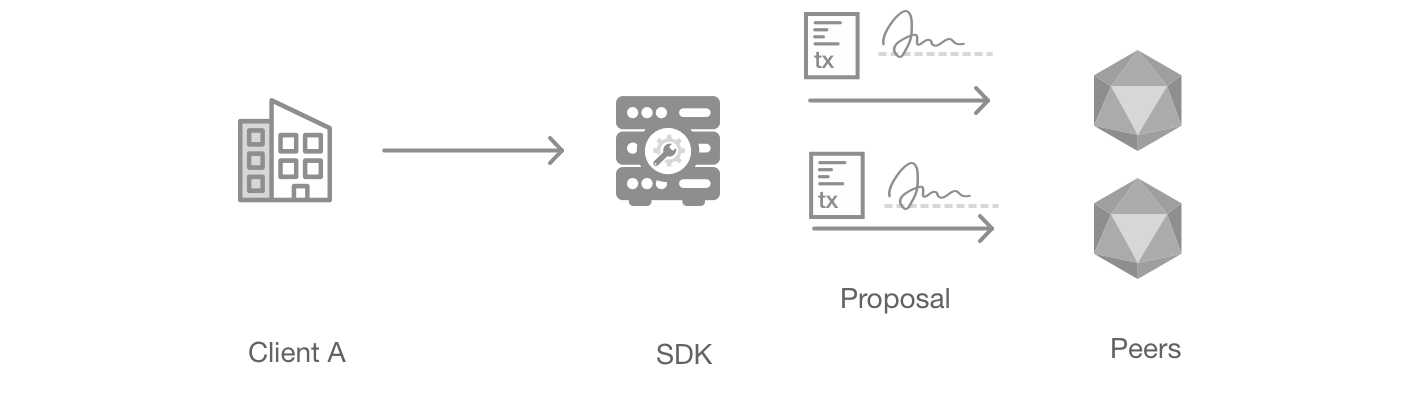
\includegraphics[width=1\textwidth]{images/4_Fabric/step1.png}
        \caption{Client creates a \acrshort{txp}.}
        \label{fig:step1}
    \end{figure}

    \item Endorsing peers simulate the transaction based on the parameters received from the client, by actually interacting with chaincode to record state updates and produce output in form of read-write set, followed by signing the read-write set and returning the results back to the client, \acrfull{txpr}.
   \begin{figure}[H]
        \centering
        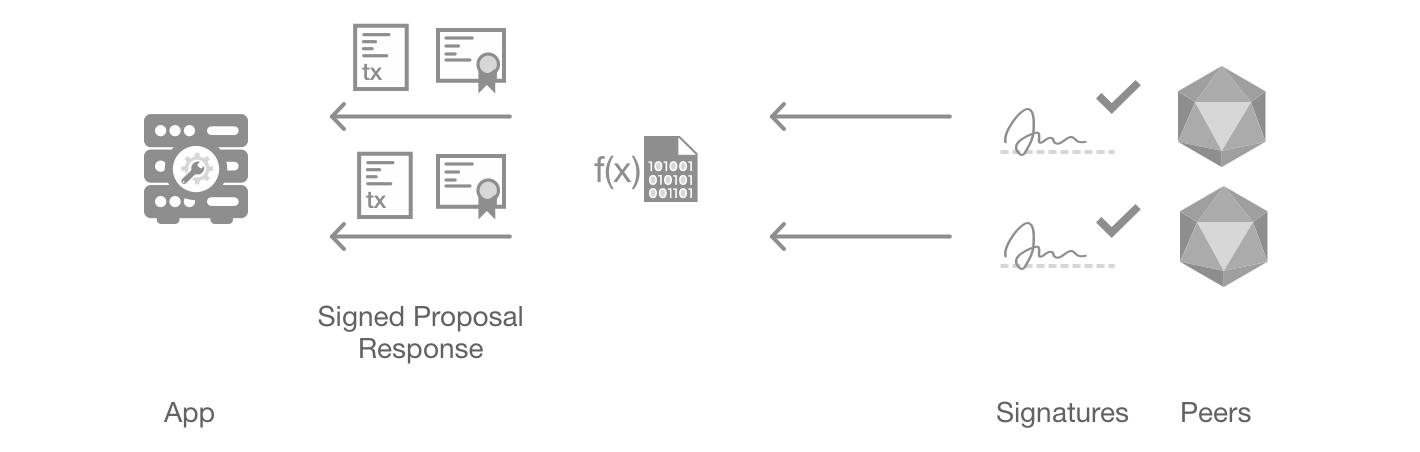
\includegraphics[width=1\textwidth]{images/4_Fabric/step2.png}
        \caption{Endorsing peers simulate and sign \acrshort{txp}.}
        \label{fig:step2}
    \end{figure}
	
    \item Client collects responses from endorsing peers, validates that results are consistent from every endorsing peer, e.g all endorsing peers have signed the same payload, followed by concatenation of all signatures of the endorsing peers along with the read-write sets, creating a transaction which is submitted to the ordering service.
    \begin{figure}[H]
        \centering
        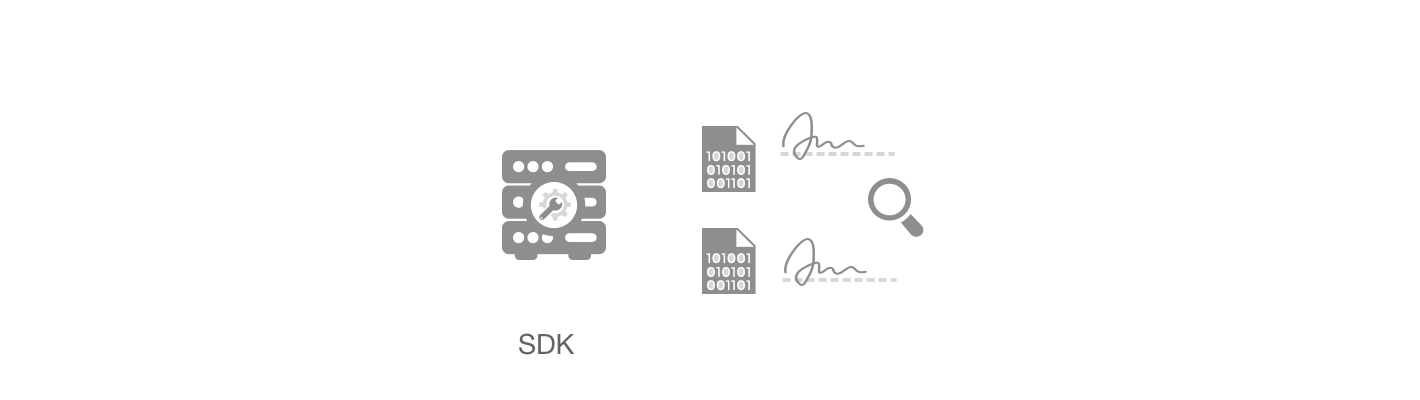
\includegraphics[width=1\textwidth]{images/4_Fabric/step3.png}
        \caption{Client collects signed \acrshort{txpr}.}
        \label{fig:step3}
    \end{figure}
    \item Ordering service collects all incoming transactions, it does not need to inspect the entire content of a transaction to perform its operation. It receives the transactions from all channels in the network, orders them chronologically by channel, and creates blocks of transactions per channel.
    \begin{figure}[H]
        \centering
        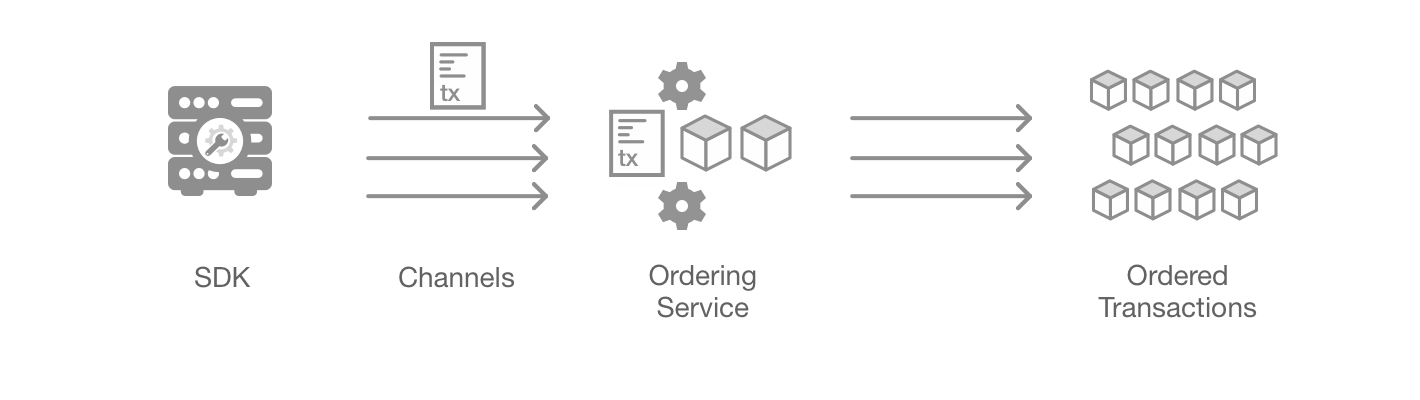
\includegraphics[width=1\textwidth]{images/4_Fabric/step4.png}
        \caption{Ordering service creates block.}
        \label{fig:step4}
    \end{figure}
    
    \item Peers of each organization, pull new blocks from the ordering service and disseminate them by using scalable middleware for ledger replication, whose implementation is based on an epidemic diffusion based protocol - gossip.
     \begin{figure}[H]
        \centering
        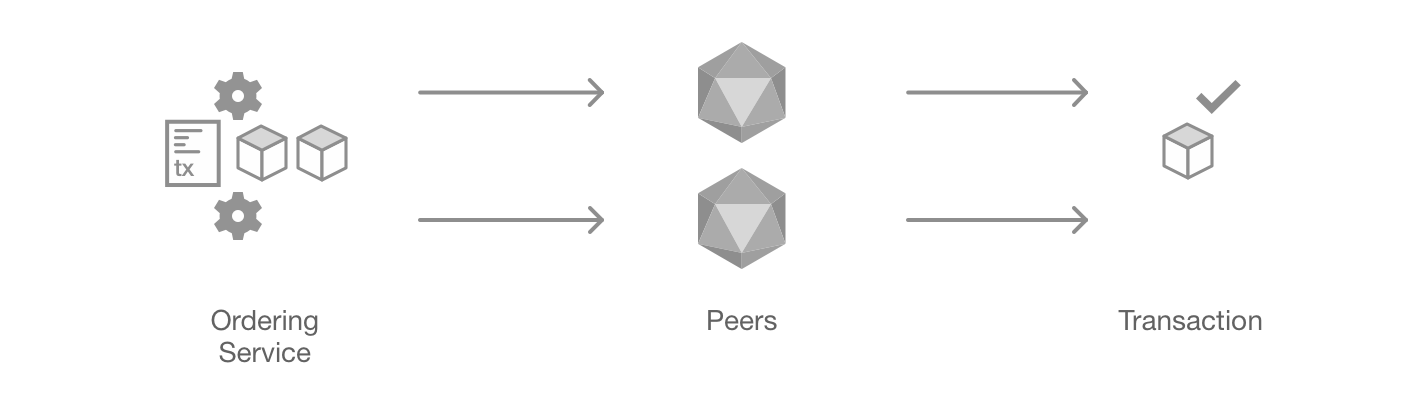
\includegraphics[width=1\textwidth]{images/4_Fabric/step5.png}
        \caption{Peers get new blocks and gossip about them.}
        \label{fig:step5}
    \end{figure}
    
    \item Each peer upon receiving a new block, iterates over transactions to:
    \begin{enumerate}
        \item validate the endorsement policy and
        \item  perform multi-value concurrency control checks.
    \end{enumerate}
    Once the transaction validation finishes, the peer appends the block to the ledger and updates its state, based on valid transactions. After the block is committed, it emits event to update the client connected to it.
    \begin{figure}[H]
        \centering
        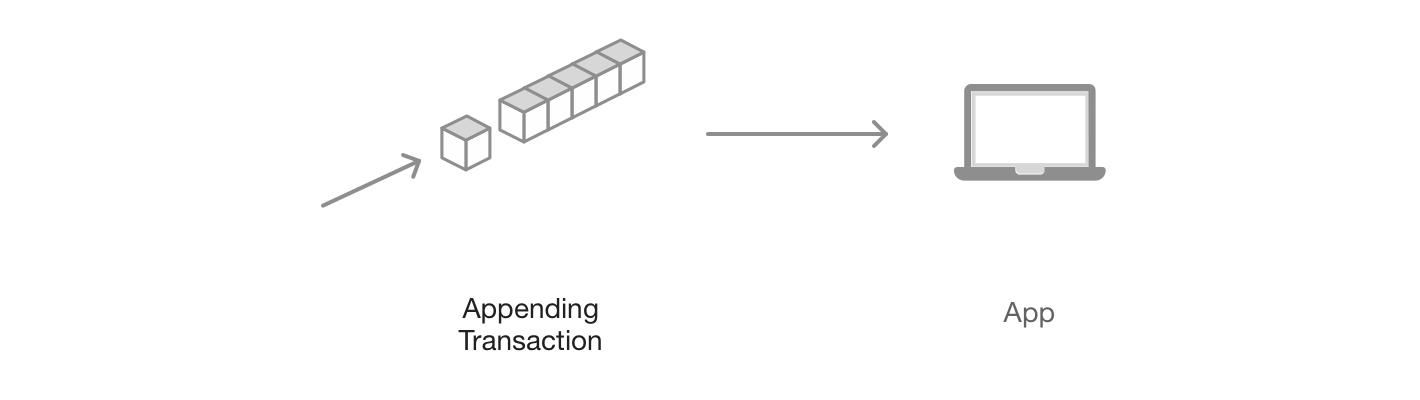
\includegraphics[width=1\textwidth]{images/4_Fabric/step6.png}
        \caption{Blocks are added to the ledger.}
        \label{fig:step6}
    \end{figure}
\end{enumerate}
Thus Fabric establishes an architecture of \textit{execute-order-validate}.
\begin{figure}[H]
        \centering
        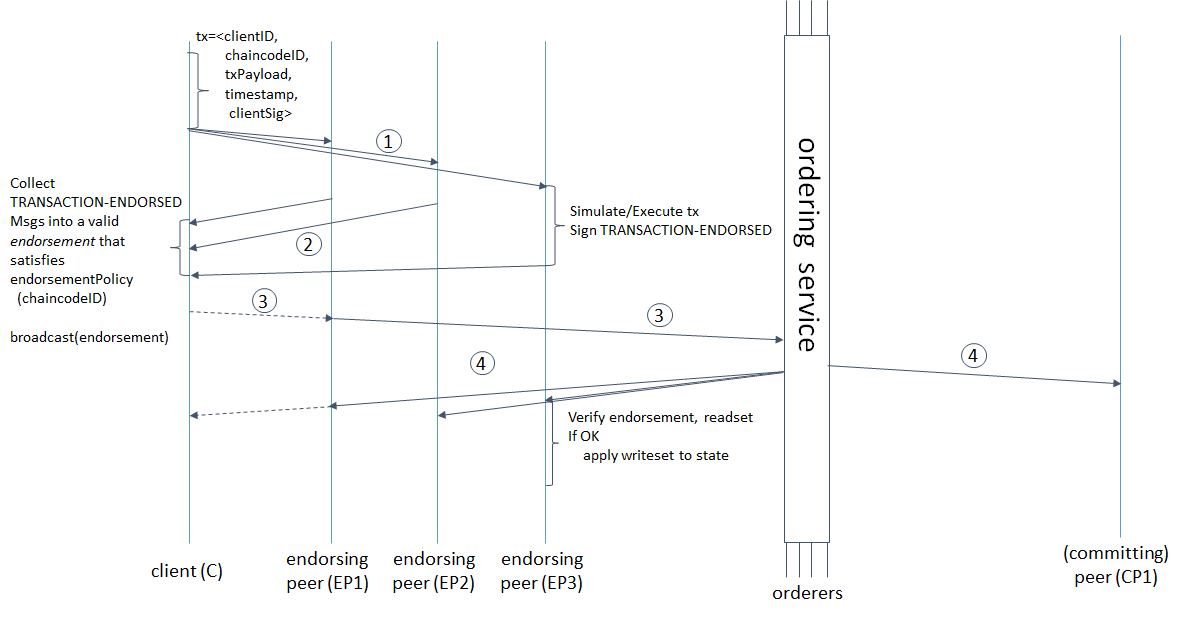
\includegraphics[width=1\textwidth]{images/4_Fabric/fabric_txFlow_normal.png}
        \caption{Flow diagram of a transaction.}
        \label{fig:tx_flox_fabric}
    \end{figure}
\subsection{Low level explanation of transaction flow}
We have two types of transactions, \textit{deploy} transactions which they create and install a new chaincode taking the program as an input, and \textit{invoke} transactions which they refer to a chaincode function for either modifying the corresponding state or returning an output read-write.

To invoke a function of a chaincode, the client sends a \verb|PROPOSE| message to a set of endorsing peers of its choice. Available endorsing peers are known by the endorsement policy of a particular \verb|chaincodeID|. If they are online, they can choose whether to endorse the transaction or not. The client has to satisfy the policy expression with the endorsers available. 

\subsection{Propose message format}
The \verb|PROPOSE| message format is \verb|<PROPOSE,tx,[anchor]>|, where \verb|tx| is mandatory. 
    \verb|tx=<clientID, chaincodeID, txPayload, timestamp, clientSig>|
    \begin{itemize}
        \item \verb|clientID|: ID of the submitting client
        \item \verb|chaincodeID|: ID of the chaincode to which the transaction is applicable to
        \item \verb|txPayload|: the payload containing the submitted transaction itself
        \item \verb|timestamp|: monotonically increasing integer for every new transaction maintained by client
        \item \verb|clientSig|: signature of client on other fields of \verb|tx|
    \end{itemize}
The details of the \verb|txPayload| differ between invoke or deploy transactions. Specifically for an invoke transaction:

    \verb|txPayload = <operation, metadata>|
    \begin{itemize}
        \item \verb|operation|: indicates the chaincode function and arguments
        \item \verb|metadata|: indicates attributes related to the invocation
    \end{itemize}
    
and for the deploy transaction:

    \verb|txPayload = <source, metadata, policies>|
    \begin{itemize}
        \item \verb|source|: indicates the source code of the chaincode
        \item \verb|metadata|: indicates attributes related to the invocation
        \item \verb|policies|: contains endorsement policy ID and its parameters for the policies related to the chaincode that are accessible to all peers.
    \end{itemize}
    
The hash of \verb|tx| is used by all nodes as a unique transaction identifier \verb|tid| and the client stores it in memory awaiting for responses from endorsing peers.


\subsection{Blockchain data structure}
% drawing of peer, endorser, committer, ledger, kvs, gossip as stack. Check Fabric OS page 8
\subsubsection{State}
The latest state of the blockchain, called World State, is modeled as a versioned key-value store (KVS). The stored data (value) and the key information for identifying the data (key) are stored as a pair. The values are stored and retrieved using a key that uniquely identifies the value and is used quickly to find the data within the database. These records are altered only by the chaincodes running on the blockchain through \verb|put| and \verb|get| KVS-operations.
State is only maintained by peers. Keys can be recognized from their name by a particular chaincode, thus they can alter only the keys that they ``possess".

\subsubsection{Ledger}
The ledger provides a verifiable history of all valid and invalid transactions, successful and unsuccessful changes to the state correspondingly. It is constructed by the ordering service as a totally ordered hash-chain of blocks. This hash-chain imposes the total order of blocks in a ledger and each block contains an array of totally ordered transactions, thus enforcing order across all transactions. Finally, every peer is responsible to maintain his ledger and it allows them to replay the history of all transactions and reconstruct the state.

\subsubsection{Block}
A block is batched, ordered transactions and contains some metadata and a link to the previous block via the block header. The main purpose of the block is to have a definite ordered entity to hash in order to include it in the next block. In figure \ref{fig:block} we present a visualization of the contents of a block.
\begin{figure}[ht]  
    \centering
    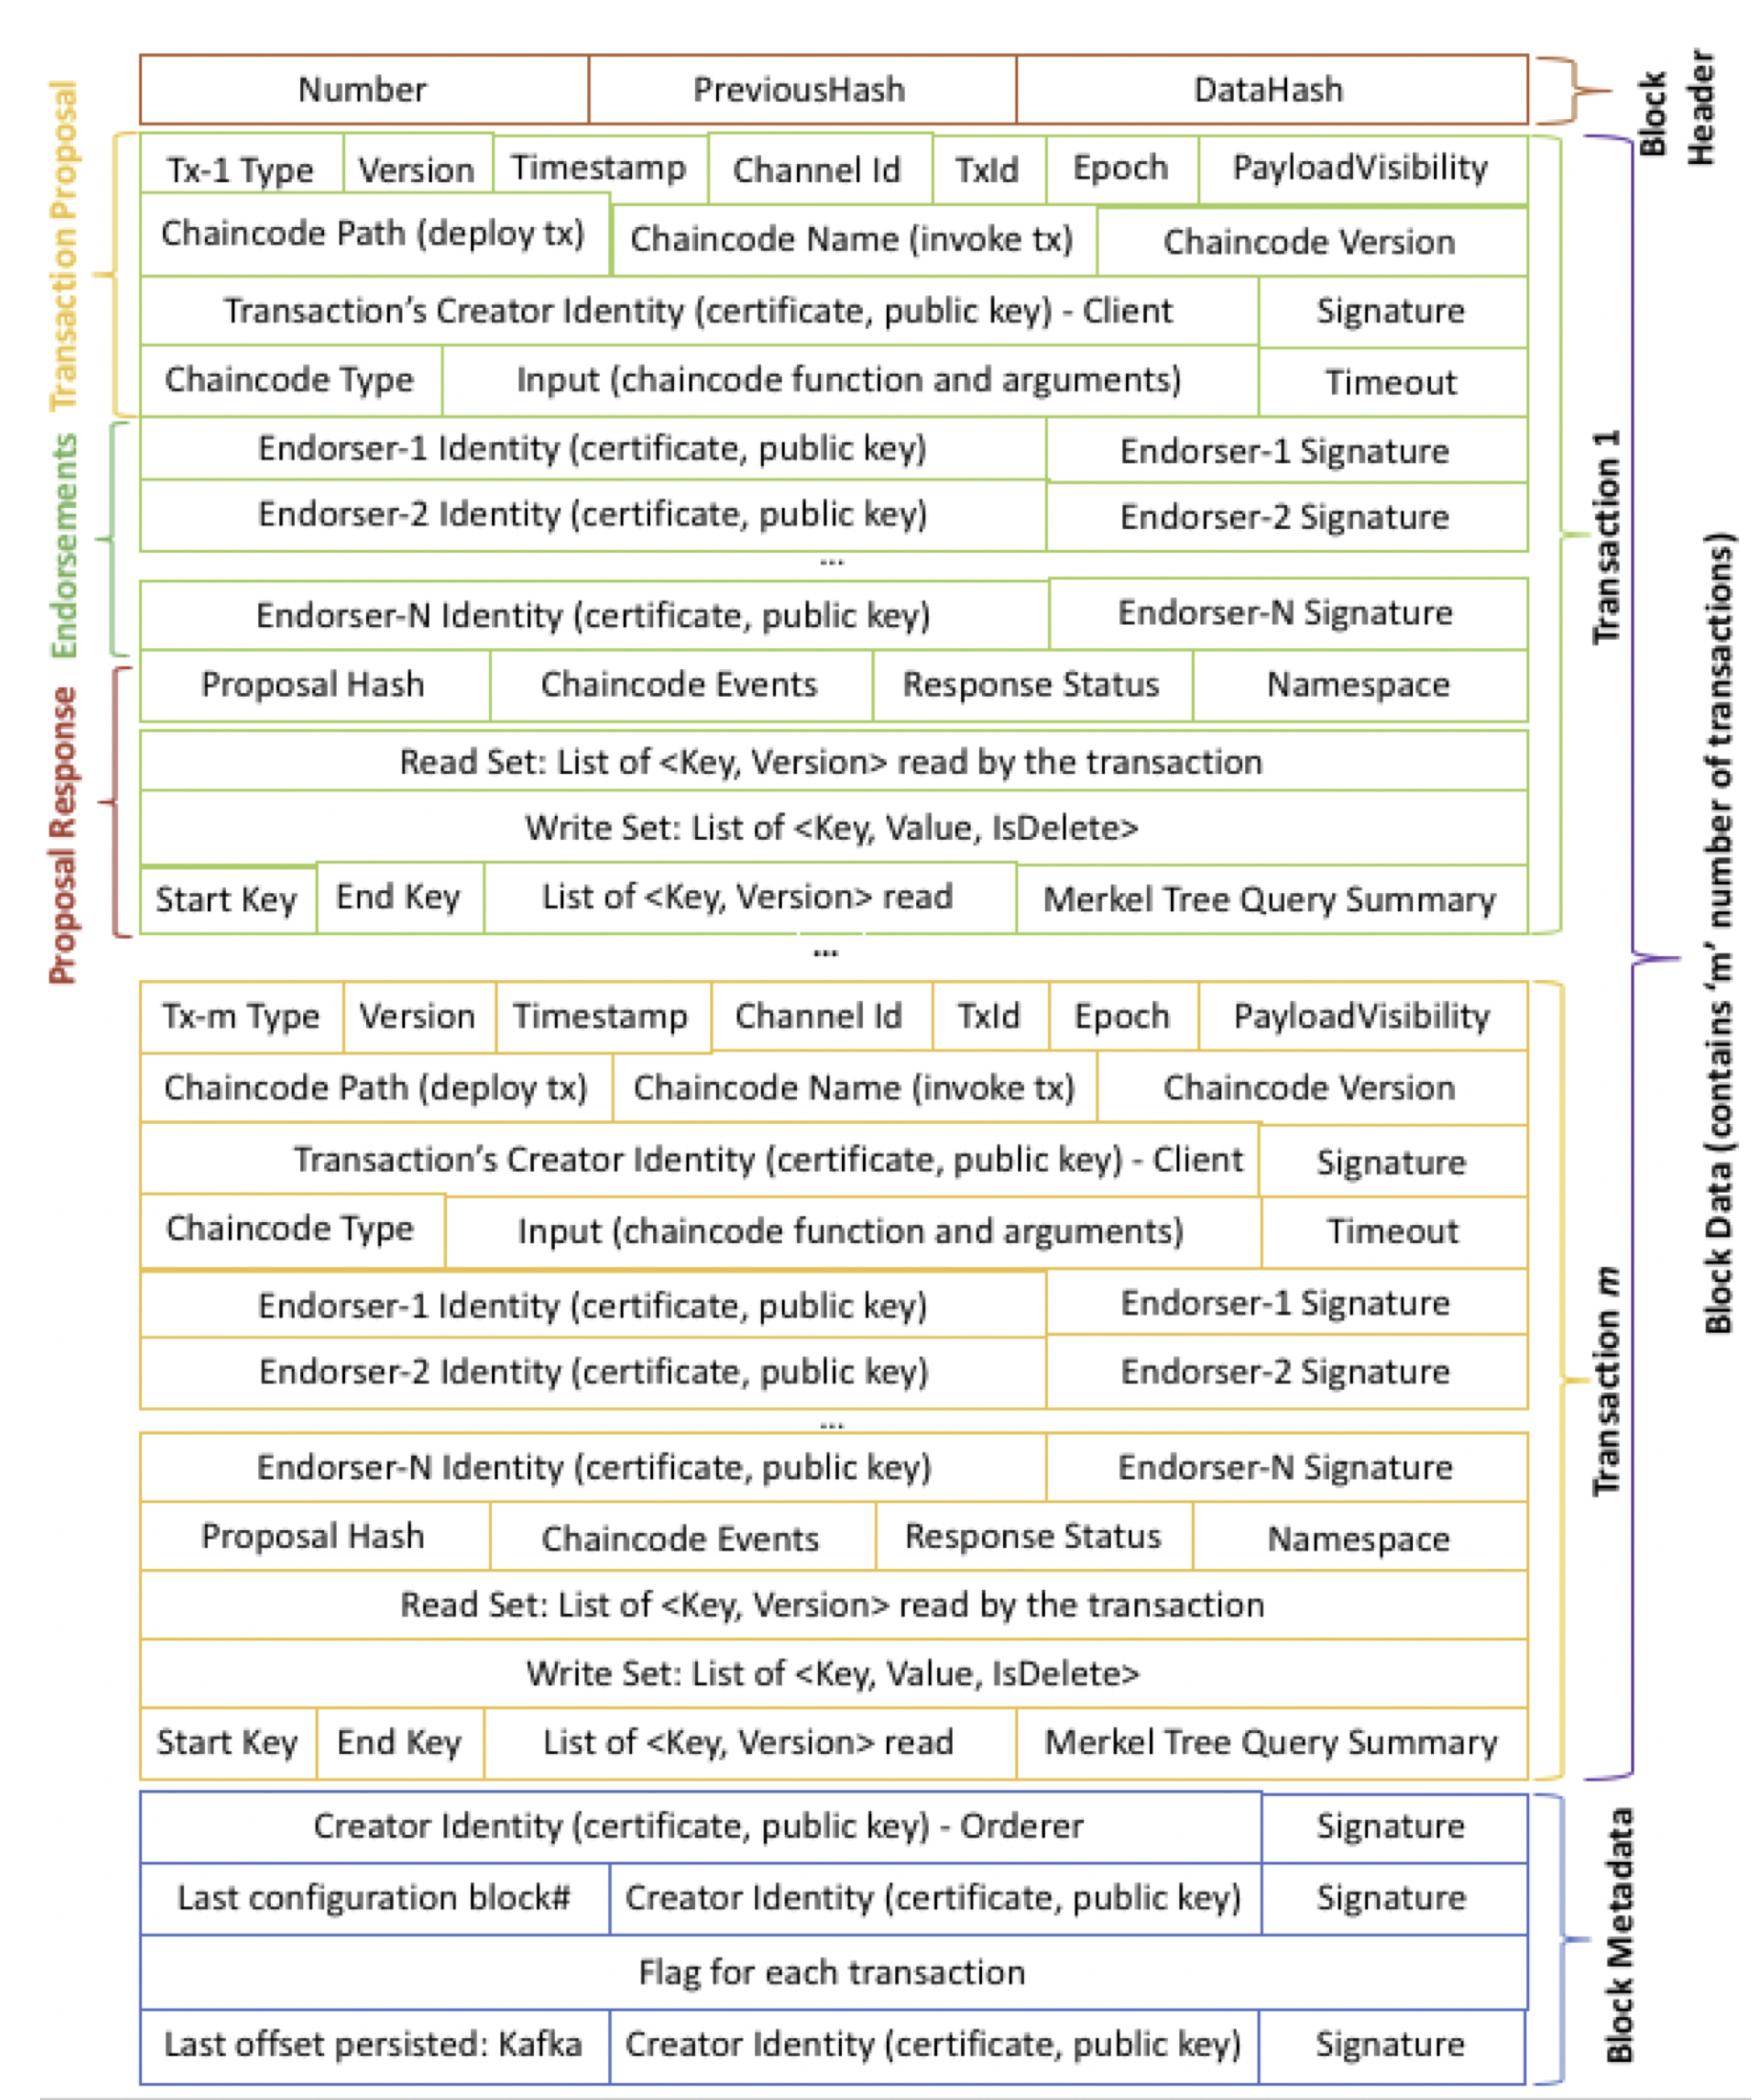
\includegraphics[width=1\textwidth]{images/4_Fabric/block.png}
    \caption{Inside a block \cite{thakkar2018performance}}
    \label{fig:block}
\end{figure}

\section{Performance}
Since we are interested in integrating IoT devices with Fabric we should elaborate on the state of Fabric's scalability, transaction throughput and performance overall. According to authors of  \cite{thakkar2018performance} and of \cite{androulaki2018hyperledger}, Fabric can achieve over 2,500 transactions per second, which should more than suffice in a permissioned set up for IoT. 
Author's of \cite{gorenflo2019fastfabric} design and implement several architectural optimizations based on common system design techniques and improve Fabric's transaction throughput by sustaining 20,000 transactions per second. 

This research points to a future Fabric that can be used as a large-scale consortium network having the capacity to handle a lot of transactions. For a perspective, VISA's network handles 24,000  \cite{visa-txs-ps}.

\section{Chaincode}
In this section, we provide a brief example of an \textit{invoke} chaincode and how a transaction would work from client's perspective.

In figure\ref{fig:examplecc} we present a basic chaincode to demo how to read/write to the ledger. It is installed on a peer and the functions in it get invoked by a client using the \acrshort{sdk}.

First, we instantiate the chaincode and we put a key-value pair for the ledger to interact with it later. Then, we construct the functions that offer the utilities needed, read and write. Mostly, they are error checking and input sanitizing code, what we are interested in is \verb|GetState| and \verb|PutState|. Those two functions read and write to ledger if everything is ok. 
% break it into to parts
Functions, starting, with a small letter are private (Golang convention), this is why we have a gateway function \verb|Invoke| that calls all the others.

Unlike Ethereum smart contracts, \acrshort{hlf} allows a continuous integration and development. The  cost to deploy a new smart contract, or update an already deployed one, is considered trivial. 
\begin{figure}
    \centering
    \lstinputlisting[language=golang]{code/examplecc.go} 
    \caption{An example chaincode demonstrating how to read and write using golang}
    \label{fig:examplecc}
\end{figure}

\begin{figure}
    \centering
    \lstinputlisting[language=golang]{code/funcscc.go}
    \caption{Callable functions of the chaincode, they define the functionality and the purpose of the chaincode}
    \label{fig:funcscc}
\end{figure}